\section{Introduction}
Benchmarking and profiling are fundamental processes for evaluating the computational performance and reliability of \acrshort{pra} tools. These processes enable the identification of performance bottlenecks, inform optimization strategies, and provide a basis for fair comparison between different quantification engines. This chapter presents a systematic benchmarking and profiling study of two PRA quantification engines: scram and SAPHSOLVE. The study uses a combination of synthetic models, the Aralia dataset, and generic Pressurized Water Reactor (PWR) models. The benchmarking methodology, performance metrics, and key findings are presented, followed by a detailed discussion of profiling results and their implications for future tool development.

\section{Benchmarking Methodology}
The benchmarking and profiling framework adopted in this study is inspired by a diagnostic methodology analogous to medical diagnostics. Just as a physician conducts an initial assessment followed by more detailed investigations, the evaluation of PRA tools begins with quick diagnostics through benchmarking, followed by detailed diagnostics via profiling. The overall workflow is illustrated in Figure~\ref{fig:diagnostic}, which serves as an overview of the approach.

\begin{figure}[h!]
    \centering
    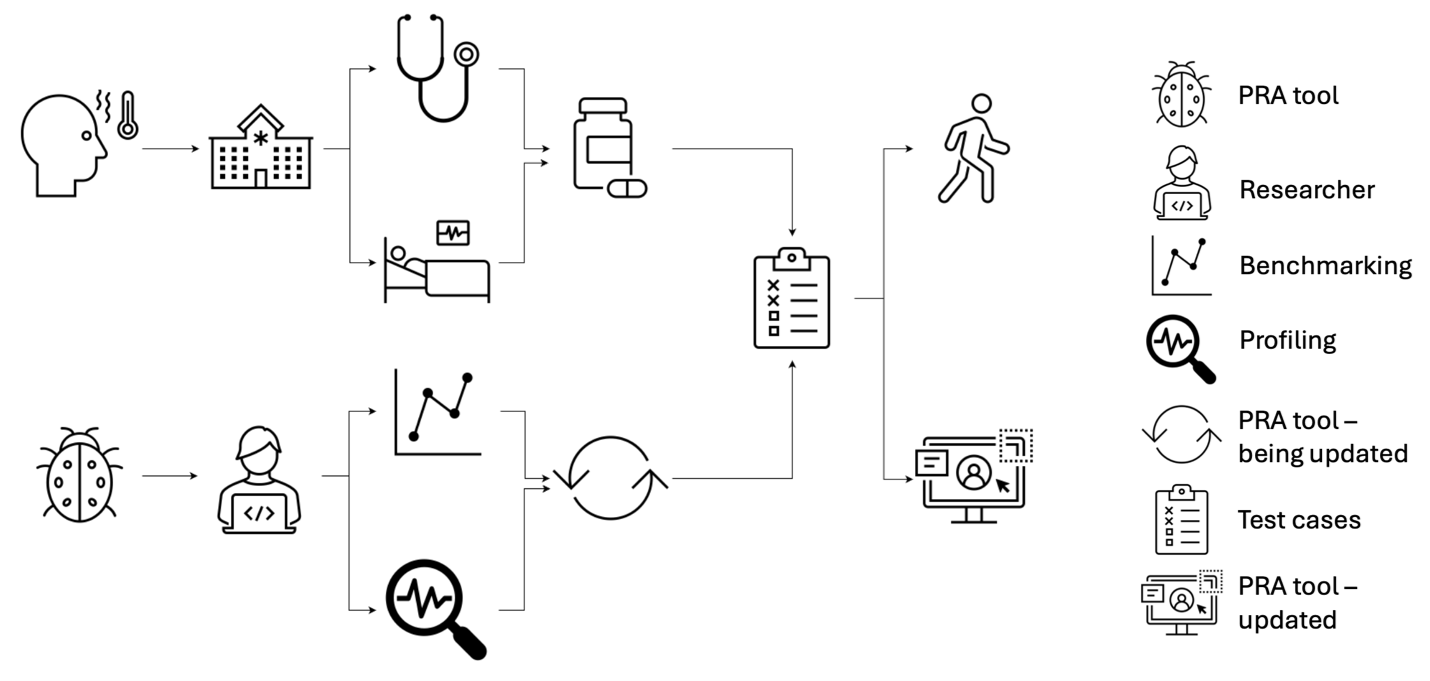
\includegraphics[width=0.9\textwidth]{3_identifying_gaps/benchmarking/profiling_methods/figures/diagnostic.png}
    \caption{Overview of diagnostic methodology for a PRA tool.}
    \label{fig:diagnostic}
\end{figure}

The benchmarking phase focuses on measuring key performance metrics such as CPU time and memory usage. However, benchmarking alone is insufficient for uncovering the root causes of inefficiency. Profiling is therefore employed to analyze the internal behavior of the code, identify computational hotspots, and guide targeted improvements. The combined outcomes of benchmarking and profiling inform an enhancement roadmap, which may include code optimization and the adoption of parallel computing strategies.

\subsection{Benchmarking Process}
The benchmarking process is structured around three essential components: the PRA model, the quantification tool, and the benchmarking configuration. Figure~\ref{fig:benchmarking_methodology} provides a schematic representation of the benchmarking methodology.

\begin{figure}[h!]
    \centering
    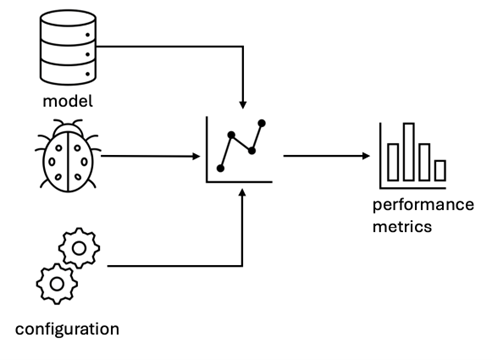
\includegraphics[width=0.5\textwidth]{3_identifying_gaps/benchmarking/profiling_methods/figures/benchmarking_methodology.png}
    \caption{Benchmarking methodology for a PRA tool.}
    \label{fig:benchmarking_methodology}
\end{figure}

Synthetic models are generated to facilitate controlled and reproducible comparisons between quantification engines. The model generator is parameterized to produce fault trees with varying numbers of basic events, gate types, and common-cause failures. Table~\ref{tab:model_generator_parameters} summarizes the key arguments and configurations used in the case study.

\begin{table}[htbp]
    \centering
    \caption{PRA model generator arguments with case study configurations.}
    \label{tab:model_generator_parameters}
    \begin{tabular}{|c|l|l|l|}
        \hline
        \textbf{Argument} & \textbf{Description} & \textbf{Option} & \textbf{Configuration} \\
        \hline
        1 & Name for fault tree & \texttt{--ft-name} & Autogenerated \\
        2 & Name for the root gate & \texttt{--root} & Root \\
        3 & Seed for PRNG & \texttt{--seed} & 123 \\
        4 & Number of basic events & \texttt{--num-basic} & 100:50:5000 \\
        5 & Average number of gate arguments & \texttt{-num-args} & 3.0 \\
        6 & Weights for gates [AND, OR, K/N, NOT, XOR] & \texttt{--weights-g} & [1,1,1,0,0] \\
        7 & Avg. \% of common basic events per gate & \texttt{--common-b} & 0.3 \\
        8 & Avg. \% of common gates per gate & \texttt{--common-g} & 0.1 \\
        9 & Avg. number of parents for common basic events & \texttt{--parents-b} & 2 \\
        10 & Avg. number of parents for common gates & \texttt{--parents-g} & 2 \\
        11 & Number of gates & \texttt{-g} or \texttt{-num-gate} & 0 \\
        12 & Maximum probability of basic events & \texttt{---max-prob} & 0.05 \\
        13 & Minimum probability of basic events & \texttt{--min-prob} & 0.01 \\
        14 & Number of house events & \texttt{--num-house} & 0 \\
        15 & Number of common-cause-failure groups & \texttt{--num-ccf} & 0 \\
        16 & Output file for the fault tree & \texttt{-o} or \texttt{-out} & XML or JSInp \\
        17 & Apply the other format to the output & \texttt{--other} & --saphsolve \\
        \hline
    \end{tabular}
\end{table}

The number of basic events is systematically varied from 100 to 5,000 in increments of 50, resulting in 99 distinct models for each engine. Gate types are randomly assigned, with AND, OR, and K/N gates occurring with equal probability. Notably, scram accepts truncation parameters via the command line, while SAPHSOLVE requires them in the input file. A probability truncation value of $10^{-20}$ is used, and no size truncation is applied. Common-cause failures, uncertainty analysis, and importance measures are excluded from this study.

The benchmarking environment is standardized to ensure fair comparison. All tools are executed with a 30-minute wall-clock time limit, 16 GB RAM, and a single CPU core. BenchExec is used to manage resource allocation and collect performance data.

\subsection{Profiling Process}
Profiling is conducted to gain deeper insight into the internal performance characteristics of the quantification engines. The profiling methodology is depicted in Figure~\ref{fig:profiling}. A challenging PRA model is selected based on benchmarking results to ensure sufficient runtime for meaningful analysis. The quantification engine is compiled in release mode with maximum optimization and debug information enabled. Intel VTune is used as the profiler due to its comprehensive analysis capabilities and user-friendly interface.

\begin{figure}[h!]
    \centering
    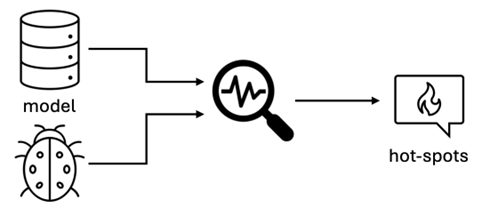
\includegraphics[width=0.5\textwidth]{3_identifying_gaps/benchmarking/profiling_methods/figures/profiling.png}
    \caption{Profiling methodology for a PRA tool.}
    \label{fig:profiling}
\end{figure}

For scram, profiling is performed on a model with 450 basic events for MOCUS MCUB, MOCUS REA, and ZBDD, and on a model with 350 basic events for BDD. For SAPHSOLVE, profiling is conducted on a model with 310 basic events, with truncation sizes varied to assess performance under different conditions. The SAPHSOLVE profiling is performed on a Windows 10 system due to observed differences in performance between the Linux and Windows versions.

\section{Benchmarking Results and Discussion}
The quick diagnostics phase evaluates the performance of scram and SAPHSOLVE across the generated synthetic models. Table~\ref{tab:quantified_input_files} summarizes the number of input files successfully quantified (out of 99 input files) by each engine and approach.

\begin{longtable}{@{}lccccc@{}}
\caption{Number of input files quantified by each engine and approach.}
\label{tab:quantified_input_files}\\
\toprule
\textbf{Approach} & \textbf{SCRAM} & \textbf{SCRAM} & \textbf{SCRAM} & \textbf{SCRAM} & \textbf{SAPHSOLVE} \\
 & \textbf{MOCUS-} & \textbf{MOCUS-} & \textbf{BDD} & \textbf{ZBDD-} & \textbf{MOCUS-} \\
 & \textbf{MCUB} & \textbf{REA} & & \textbf{REA} & \textbf{MCUB} \\
\midrule
\endfirsthead
\toprule
\textbf{Approach} & \textbf{SCRAM} & \textbf{SCRAM} & \textbf{SCRAM} & \textbf{SCRAM} & \textbf{SAPHSOLVE} \\
 & \textbf{MOCUS-} & \textbf{MOCUS-} & \textbf{BDD} & \textbf{ZBDD-} & \textbf{MOCUS-} \\
 & \textbf{MCUB} & \textbf{REA} & & \textbf{REA} & \textbf{MCUB} \\
\midrule
\endhead
\midrule
\endfoot
\bottomrule
\endlastfoot
Quantified files & 89 & 89 & 3 & 90 & 82 \\
\end{longtable}

The results indicate that the MOCUS and ZBDD algorithms in scram, as well as the MOCUS algorithm in SAPHSOLVE, are able to quantify the majority of models. The BDD approach in scram is limited by high memory requirements, resulting in only three successful quantifications. Models that cannot be quantified typically fail during the cut set generation step. For example, the ft-1300 model requires adjustment of the limit order in the size of minimal cut sets (MCS) to complete quantification. The relationship between the limit order and quantification time is exponential, as illustrated in Figure~\ref{fig:ft_1300}.

\begin{figure}[h!]
    \centering
    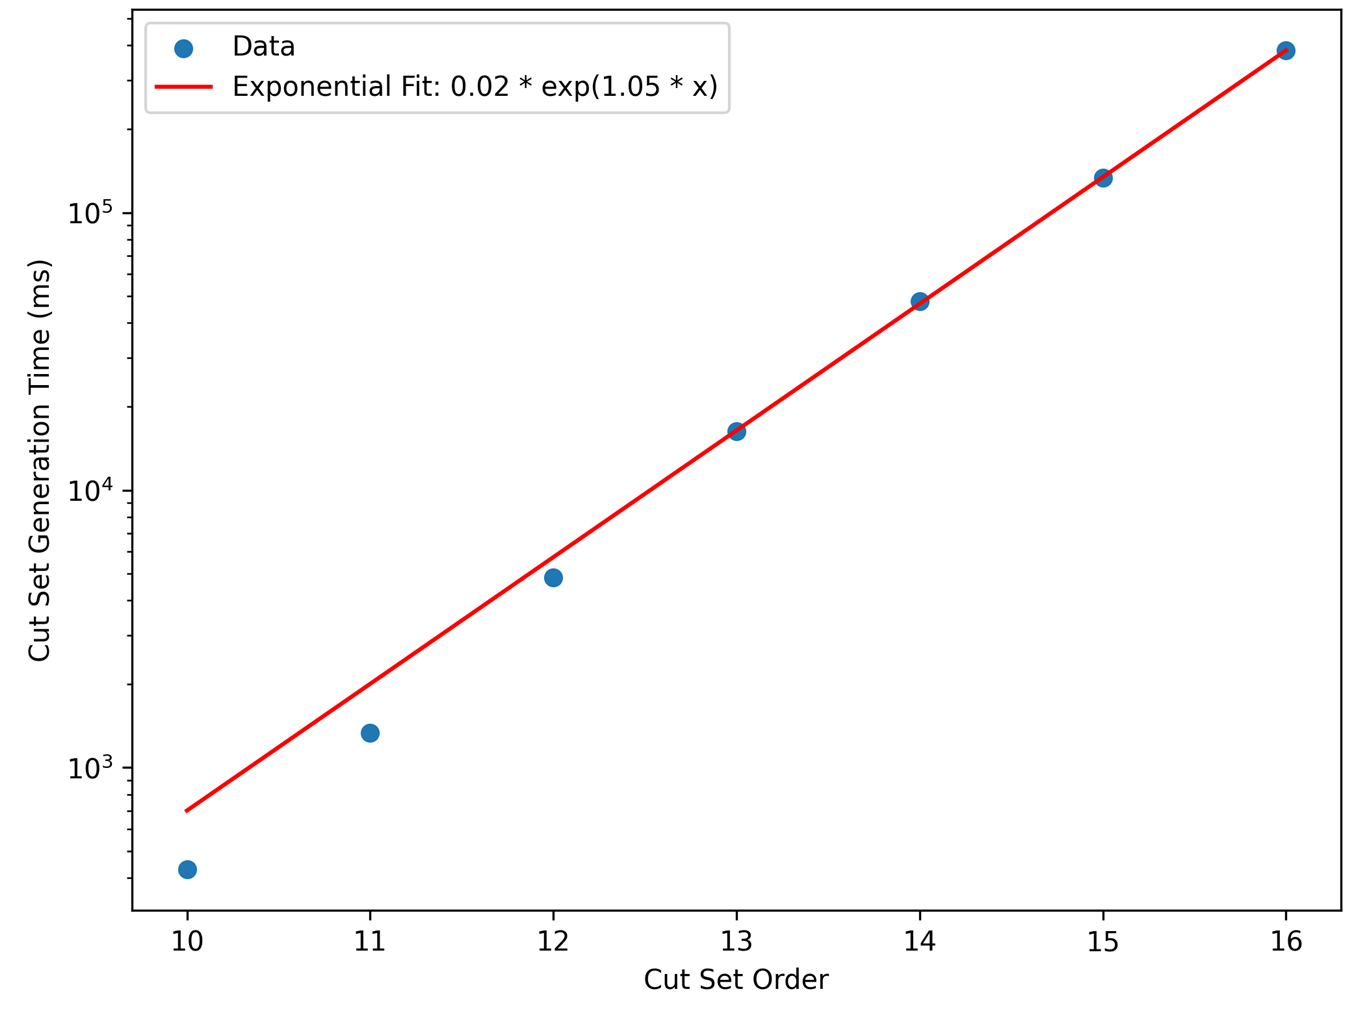
\includegraphics[width=0.75\textwidth]{3_identifying_gaps/benchmarking/profiling_methods/figures/ft_1300.png}
    \caption{Effect of limit order on MCS of scram for ft-1300 model.}
    \label{fig:ft_1300}
\end{figure}

A comparison of the number of cut sets generated by scram and SAPHSOLVE reveals that, in most cases, the results are consistent. However, differences are observed in a few models, particularly when using the ZBDD approach in scram. The probability results obtained by scram-MOCUS-MCUB and SAPHSOLVE-MOCUS-MCUB are identical, providing a valuable cross-check between the two engines.

The quantification time for scram is approximately linear with respect to the number of cut sets generated, as shown in Figure~\ref{fig:scram_quant_time}. While most models are quantified within the time limit, some require up to 20 minutes, which is not acceptable for practical PRA applications. The ZBDD approach is significantly faster than MOCUS, and BDD is the fastest when sufficient resources are available.

\begin{figure}[h!]
    \centering
    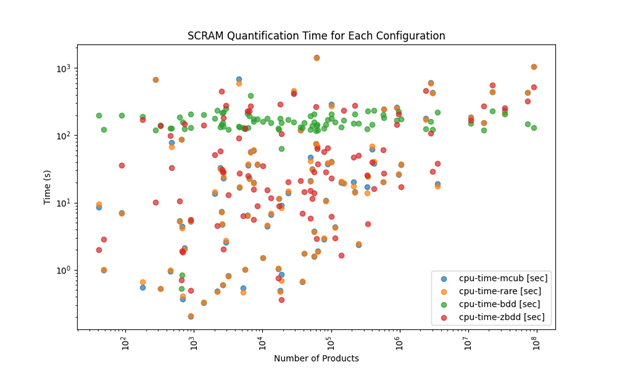
\includegraphics[width=0.9\textwidth]{3_identifying_gaps/benchmarking/profiling_methods/figures/scram_quant_time.png}
    \caption{scram quantification time results for all approaches.}
    \label{fig:scram_quant_time}
\end{figure}

Memory usage in scram increases with model size, as depicted in Figure~\ref{fig:scram_memory_usage}. BDD runs are generally infeasible due to excessive memory demands. The flat line in the figure represents the predefined memory limit.

\begin{figure}[H]
    \centering
    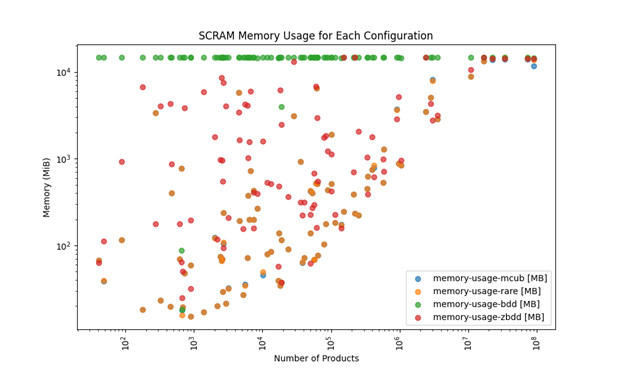
\includegraphics[width=0.9\textwidth]{3_identifying_gaps/benchmarking/profiling_methods/figures/scram_memory_usage.png}
    \caption{scram memory usage for all approaches.}
    \label{fig:scram_memory_usage}
\end{figure}

SAPHSOLVE quantifies 82 out of 99 models using the MOCUS approach with MCUB probability approximation. Its quantification time is consistently low, as shown in Figure~\ref{fig:saphsolve_quant_time}, due to early termination and efficient resource management. However, the Linux version of SAPHSOLVE is less capable than the Windows version when running without truncation.

\begin{figure}[H]
    \centering
    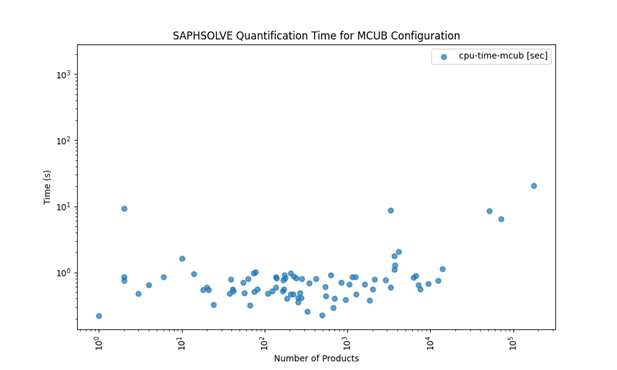
\includegraphics[width=0.9\textwidth]{3_identifying_gaps/benchmarking/profiling_methods/figures/saphsolve_quant_time.png}
    \caption{SAPHSOLVE quantification time results for MOCUS MCUB.}
    \label{fig:saphsolve_quant_time}
\end{figure}

SAPHOLVE's memory usage is also efficient, as depicted in Figure~\ref{fig:saphsolve_memory_usage}. The number of cut sets generated is slightly lower than in scram, which contributes to faster results.

\begin{figure}[H]
    \centering
    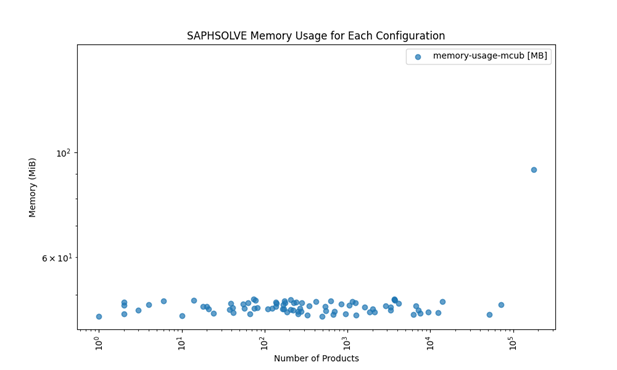
\includegraphics[width=0.9\textwidth]{3_identifying_gaps/benchmarking/profiling_methods/figures/saphsolve_memory_usage.png}
    \caption{SAPHSOLVE memory usage for MOCUS MCUB.}
    \label{fig:saphsolve_memory_usage}
\end{figure}

The benchmarking results highlight the trade-offs between speed, memory usage, and output detail. scram provides more detailed output but at the cost of higher resource consumption, while SAPHSOLVE is optimized for speed and minimal output.

\section{Profiling Results and Discussion}
Profiling provides detailed diagnostics of the quantification engines, enabling the identification of computational hotspots and inefficiencies. The profiling setup differs between scram and SAPHSOLVE due to differences in model formats, programming languages, and operating environments.

\subsection{scram Profiling}
Table~\ref{tab:scram_profiling} summarizes the profiling results for scram across different quantification approaches and input files.

\begin{table}[htbp]
    \centering
    \caption{Summary of profiling performance analysis results for scram.}
    \label{tab:scram_profiling}
    \begin{tabular}{|l|c|c|c|c|}
        \hline
        \textbf{Approach} & \textbf{MOCUS-} & \textbf{MOCUS-} & \textbf{BDD} & \textbf{ZBDD-} \\
        \textbf{-Approximation} & \textbf{MCUB} & \textbf{REA} & & \textbf{REA} \\
        \hline
        Input File & ft-450 & ft-450 & ft-350 & ft-450 \\
        Analysis Time [sec] & 431.230 & 426.177 & 62.566 & 320.072 \\
        Core Utilization & 0.972 out of 6 & -- & -- & -- \\
        \hline
    \end{tabular}
\end{table}

Hot spot analysis reveals that result reporting and cut set generation dominate computation time for the MOCUS and ZBDD algorithms. BDD construction is the primary bottleneck for the BDD approach. Figures~\ref{fig:vtune_scram_mocus_mcub} through~\ref{fig:vtune_scram_zbdd} provide VTune profiling results for each approach.

\begin{figure}[H]
    \centering
    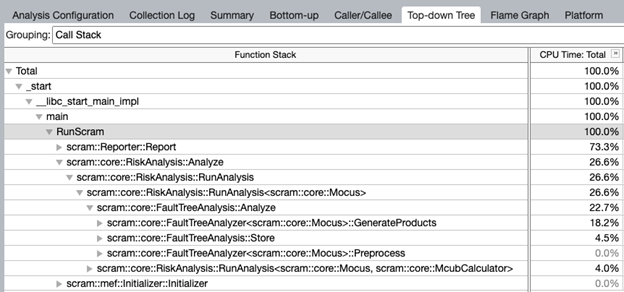
\includegraphics[width=0.9\textwidth]{3_identifying_gaps/benchmarking/profiling_methods/figures/vtune_scram_mocus_mcub.png}
    \caption{scram MOCUS MCUB VTune profiling results.}
    \label{fig:vtune_scram_mocus_mcub}
\end{figure}

\begin{figure}[H]
    \centering
    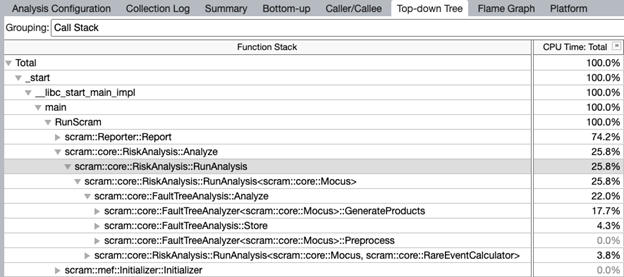
\includegraphics[width=0.9\textwidth]{3_identifying_gaps/benchmarking/profiling_methods/figures/vtune_scram_mocus_rea.png}
    \caption{scram MOCUS REA VTune profiling results.}
    \label{fig:vtune_scram_mocus_rea}
\end{figure}

\begin{figure}[H]
    \centering
    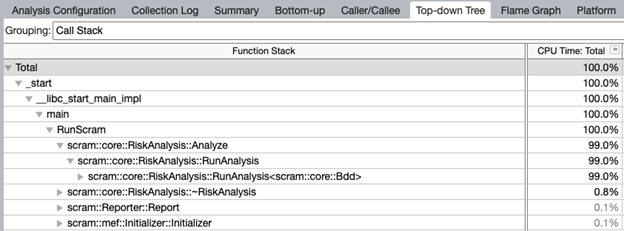
\includegraphics[width=0.9\textwidth]{3_identifying_gaps/benchmarking/profiling_methods/figures/vtune_scram_bdd.png}
    \caption{scram BDD VTune profiling results.}
    \label{fig:vtune_scram_bdd}
\end{figure}

\begin{figure}[H]
    \centering
    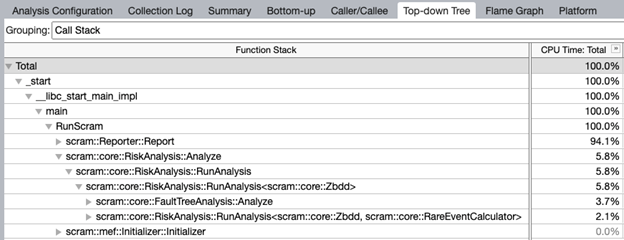
\includegraphics[width=0.9\textwidth]{3_identifying_gaps/benchmarking/profiling_methods/figures/vtune_scram_zbdd.png}
    \caption{scram ZBDD REA VTune profiling results.}
    \label{fig:vtune_scram_zbdd}
\end{figure}

\subsection{SAPHSOLVE Profiling}
Table~\ref{tab:saphsolve_profiling} presents the profiling results for SAPHSOLVE at different truncation sizes.

\begin{table}[htbp]
    \centering
    \caption{Summary of profiling performance analysis results for SAPHSOLVE.}
    \label{tab:saphsolve_profiling}
    \begin{tabular}{|l|c|c|c|}
        \hline
        \textbf{Truncation Size} & 16 & 18 & 20 \\
        \hline
        Input File Configuration & ft-310 & ft-310 & ft-310 \\
        Analysis Elapsed Time [sec] & 361.010 & 4,142.099 & 64,365.847 \\
        Number of Cut Sets & 11,490 & 102,444 & 761,472 \\
        Probability & $1.3388 \times 10^{-11}$ & -- & -- \\
        Physical Core Utilization & 1.306 out of 4 & -- & -- \\
        \hline
    \end{tabular}
\end{table}

The relationship between truncation size and calculation time in SAPHSOLVE is exponential, as shown in Figure~\ref{fig:saphsolve_truncation_time}. For large truncation sizes, performance degrades significantly, indicating a need for optimization in the size truncation implementation.

\begin{figure}[H]
    \centering
    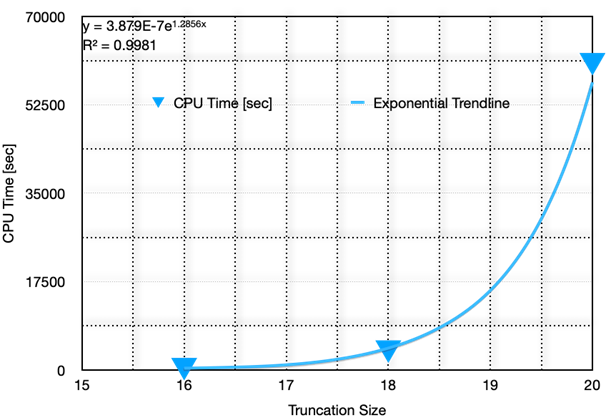
\includegraphics[width=0.8\textwidth]{3_identifying_gaps/benchmarking/profiling_methods/figures/saphsolve_truncation_time.png}
    \caption{SAPHSOLVE quantification time for different truncation sizes.}
    \label{fig:saphsolve_truncation_time}
\end{figure}

Table~\ref{tab:saphsolve_vtune} summarizes the VTune profiling results for SAPHSOLVE, highlighting the dominant functions and their contribution to total runtime.

\begin{table}[htbp]
    \centering
    \caption{SAPHSOLVE MOCUS MCUB VTune profiling results.}
    \label{tab:saphsolve_vtune}
    \begin{tabular}{|c|c|c|c|}
        \hline
        \textbf{Truncation Size} & \textbf{Function} & \textbf{CPU Time [sec]} & \textbf{Percentage Contribution [\%]} \\
        \hline
        16 & A & 175.643 & 49.5 \\
           & B & 52.284 & 14.7 \\
        18 & B & 1648.13 & 43 \\
           & A & 708.83 & 18.5 \\
        20 & B & 43893.54 & 72.2 \\
           & C & 3929.234 & 6.5 \\
           & A & 3580.815 & 5.9 \\
        \hline
    \end{tabular}
\end{table}

Functions responsible for cut set generation dominate the runtime, especially as truncation size increases. This observation underscores the importance of efficient cut set management in large scale PRA quantification.

\section{Conclusion}
Benchmarking and profiling are indispensable for the rigorous evaluation and improvement of PRA quantification engines. The results presented in this chapter demonstrate that while both scram and SAPHSOLVE are capable of quantifying large synthetic models, their performance characteristics differ significantly. scram offers detailed output and multiple quantification approaches but at the cost of higher resource consumption. SAPHSOLVE is optimized for speed and minimal output but exhibits performance degradation for large truncation sizes. Profiling reveals that cut set generation is the primary computational bottleneck in both engines. These insights provide a foundation for targeted optimization and future development of high performance PRA tools.

\section{Transformations}
\subsection{Knowledge Compilation}
Casting \acrshort{pra} model as \acrshort{pdag} allows to view the model a set of boolean propositional statements. Thus, any question that can be asked about the system, can be seen as a general reasoning (queries or transformations) over the knowledge base, defined by the propositional statements. A common approach to dealing with such problems is knowledge compilation.

Knowledge Compilation has emerged as a significant direction of research for addressing the computational intractability inherent in general propositional reasoning tasks. This approach, which has a long tradition in reasoning Artificial Intelligence, was notably structured and analyzed in the work of Darwiche and Marquis. KC fundamentally involves splitting the reasoning process into two distinct phases:
\begin{enumerate}
    \item An \textbf{off-line compilation phase}: In this initial phase, a knowledge base (represented, for instance, as a propositional theory or formula) is transformed or "compiled" into a different representation, referred to as a tractable form, or target language. The target language is specifically chosen because it supports certain desirable properties, such as tractability for specific queries (questions) or allowing polynomial time evaluation.
    \item An \textbf{on-line query-answering phase}: Once compiled, the resulting target representation is utilized to answer queries efficiently. The goal is for these query answering procedures to be polynomial time with respect to the size of the compiled representation.
\end{enumerate}
The primary rationalization behind this two-phase approach is to \textbf{shift as much of the computational overhead as possible into the off-line compilation phase}. While the compilation step itself can be computationally hard, this initial cost is amortized over the potentially large number of subsequent on-line queries. This amortized cost makes the overall reasoning process more efficient when multiple queries are anticipated on the same knowledge base.

\subsection{Negation Normal Form (NNF)}
The field of knowledge compilation operates primarily on a subset of boolean expression that conform to a set of properties. In general, imposition of more properties results increased tractability of the queries, i.e. answering questions becomes easier, however, at the cost of the size of boolean expression. The primary ``workhorse'' of Knowledge compilation is \acrfull{nnf}.

Boolean \acrfull{nnf} is a syntactic restriction for Boolean formulas such that negations (NOT operators) are applied only directly to variables and not to compound subformulas. Formally, a Boolean formula is in \acrshort{nnf} if it is built from variables, their negations, conjunctions (AND), and disjunctions (OR), where NOT appears only as part of literals.

A boolean expression in \acrshort{nnf} can be represented as a rooted directed acyclic graph, \acrshort{dag}. The leaf of the graph correspond to constants (0, 1) or literals ($a$, $\neg b$), presented in the expression. The internal nodes of the \acrshort{dag} correspond to AND ($\land$) and OR ($\lor$) gates. Internal gates cannot be associated with NOT gates.

In the context of knowledge compilation, \acrshort{nnf} serves as a foundational target language. Knowledge bases compiled into \acrshort{nnf} allow efficient model checking and form the basis for further restricted normal forms like \acrfull{cnf}, \acrfull{dnf}, \acrfull{dnnf}, or \acrfull{d-dnnf}. \acrshort{nnf} enables subsequent transformations and reasoning tasks to be performed with well-bounded complexity, as it ensures logical negation is ``pushed down'' to the leaves of the formula's parse tree, simplifying subsequent manipulations.

\subsubsection{Properties of NNF}
 \acrshort{nnf}s can be classified based on adherence to particular properties/restrictions. The set of  \acrshort{nnf}s that adhere to a set of properties defines a representational language, $L$ in Table \ref{tbl:kc_language_properties}.

\paragraph{Decomposability}
An \acrshort{nnf} is decomposable if, at every conjunction ($\land$) gate, the sets of variables feeding into the subformulas of its children are pairwise disjoint. That is, for any $\wedge$-node with children, the sets of variables involved in the subformulas rooted at those children share no variables. 
Formally, for any $\wedge$-node with children ($\alpha_1, \ldots, \alpha_n$),
\[
\mathrm{Vars}(\alpha_i) \cap \mathrm{Vars}(\alpha_j) = \emptyset \quad \forall i \neq j
\]
This property ensures tractable consistency checking and supports efficient computation on the representation. The language of \acrshort{dnnf} comprises those \acrshort{nnf}s that are decomposable.

\paragraph{Determinism}
An \acrshort{nnf} is deterministic if, at every disjunction ($\lor$) gate, the sets of models (i.e., assignments that make the subformulas true) computed by its children are mutually exclusive--no single assignment satisfies more than one child. 
Zero-overlap of assignments between children guarantees tractable model counting. Determinism together with decomposability yields \acrfull{d-dnnf}, which enables polytime validity, implicant, and model counting queries. \acrfull{sdd}s are a strict subset of \acrshort{d-dnnf} with additional structure.

\paragraph{Smoothness}
An \acrshort{nnf} is smooth if, at every disjunction ($\lor$) gate, all children depend on the same set of variables (atoms). That is, for every OR-node, the set of variables in each child's subformula is identical. Smoothness simplifies certain operations in knowledge compilation and ensures that the models of disjuncts are over a fixed set of variables. Smoothness can always be enforced on any \acrshort{dnnf} in polynomial time without affecting succinctness. \acrfull{sd-dnnf} enforces decomposability, determinism, and smoothness.

\paragraph{Flatness}
An \acrshort{nnf} is flat if the circuit/tree has height at most two: the root is an AND or OR, and the children are literals or simple conjunction/disjunctions of literals. Both \acrshort{cnf} and \acrshort{dnf} are examples of \acrfull{f-nnf}: In \acrshort{cnf}, the root is AND, its children are ORs of literals (clauses); in \acrshort{dnf}, the root is OR, its children are ANDs of literals (terms). Flatness restricts structural complexity and further subclasses are defined by additional properties: for instance, \acrshort{cnf} requires each clause to have no repeated variables, and \acrshort{dnf} requires each term to have unique variables.

\subsubsection{Summary}
The following sections explore common target languages that find uses in Knowledge Compilation and can be used in \acrshort{pra}. For each selected language we note it's main properties, construction algorithms, and tractable queries available for this languages. We focus on the following:
\begin{enumerate}
    \item \acrshort{cnf} --- the most well-studied form, ubiquitous in solving SAT problem.
    \item \acrshort{dnf} --- a form that naturally renders itself for \acrlong{et} analysis and acts as a precursor for more sophisticated essential prime implicant search.
    \item \acrshort{bdd}, \acrshort{zdd}, \acrshort{sdd} --- most tractable target languages, featured in the majority of practical applications.
\end{enumerate}
This is not an exhaustive list. It's intention is to provide a summary of rigorous formalism that can find uses in \acrfull{pra}.

\begin{figure}[ht!]
\centering
\begin{tikzpicture}
\tikzset{canonical/.style={fill=blue!30},myedges/.style={-, >={Stealth[reversed]}, thick},anchored/.style={draw=none, opacity=0, font=\tiny}}
\graph [layered layout, nodes=draw, edges=rounded corners,edge=myedges] {
{[edge={draw=none},nodes=anchored]
1 -> 2 -> 3 -> 4 -> 5 -> 6 -> 7 -> 8 -> 9 -> 10;
};
{ [same layer] 1, "Boolean Expression" },
{ [same layer] 2, NNF, XAG},
{ [same layer] 3, "f-NNF", DNNF, "d-NNF", AIG, RNF},
{ [same layer] 4, CNF, DNF, "s-DNNF", "d-DNNF", FPRM },
{ [same layer] 5, PI[canonical], "IP/BCF"[canonical], PPRM[canonical]},
{ [same layer] 6, EPI[canonical], EIP[canonical] },
{ [same layer] 7, "sd-DNNF", BDD },
{ [same layer] 8, "f-BDD" },
{ [same layer] 9, OBDD },
{ [same layer] 10, SDD[canonical], ROBDD[canonical] },

{NNF, XAG} -> "Boolean Expression",
{AIG, RNF} -> XAG,
{"f-NNF", DNNF, "d-NNF"} -> NNF,
{CNF, DNF} -> "f-NNF",
PI -> CNF,
EPI -> PI,
"IP/BCF" -> DNF,
EIP -> "IP/BCF",
{DNF, "s-DNNF", "d-DNNF"} -> DNNF,
"d-DNNF" -> "d-NNF",
BDD -> "d-DNNF",
"f-BDD" -> BDD,
ROBDD -> OBDD,
OBDD -> "f-BDD",
SDD -> "sd-DNNF",
"sd-DNNF" -> {"s-DNNF", "d-DNNF"},
FPRM -> RNF,
PPRM -> FPRM,
};
\end{tikzpicture}
\caption[Hierarchy of compiled target languages.]{Hierarchy of compiled target languages. Blue nodes represent canonical forms.}
\end{figure}

\begin{longtable}[ht!]{ll}
\caption{Compiled target languages, acronyms defined.} \\
\toprule
\textbf{Acronym} & \textbf{Full form} \\
\midrule
\endfirsthead

\multicolumn{2}{c}{\textit{Continued: Compiled target languages, acronyms defined.}} \\
\toprule
\textbf{Acronym} & \textbf{Full form} \\
\midrule
\endhead

\endfoot
\bottomrule
\endlastfoot

\acrshort{nnf}    & \acrlong{nnf}    \\
\acrshort{xag}    & \acrlong{xag}    \\
\acrshort{aig}    & \acrlong{aig}    \\
\acrshort{rnf}    & \acrlong{rnf}    \\
\acrshort{f-nnf}  & \acrlong{f-nnf}  \\
\acrshort{dnnf}   & \acrlong{dnnf}   \\
\acrshort{d-nnf}  & \acrlong{d-nnf}  \\
\acrshort{fprm}   & \acrlong{fprm}   \\
\acrshort{cnf}    & \acrlong{cnf}    \\
\acrshort{dnf}    & \acrlong{dnf}    \\
\acrshort{s-dnnf} & \acrlong{s-dnnf} \\
\acrshort{d-dnnf} & \acrlong{d-dnnf} \\
\acrshort{sd-dnnf} & \acrlong{sd-dnnf} \\
\acrshort{pprm}   & \acrlong{pprm}   \\
\acrshort{pi}     & \acrlong{pi}     \\
\acrshort{ip}     & \acrlong{ip}     \\
\acrshort{bcf}     & \acrlong{bcf}     \\
\acrshort{epi}    & \acrlong{epi}    \\
\acrshort{eip}    & \acrlong{eip}    \\
\acrshort{bdd}    & \acrlong{bdd}    \\
\acrshort{f-bdd}  & \acrlong{f-bdd}  \\
\acrshort{obdd}   & \acrlong{obdd}   \\
\acrshort{sdd}    & \acrlong{sdd}    \\
\acrshort{robdd}  & \acrlong{robdd}  \\
\end{longtable}

\begin{landscape}
\begin{longtable}{@{}lccccccc@{}}
\caption[Properties of selected target languages.]{Properties of selected target languages.}
\label{tbl:kc_language_properties}\\
\toprule
\textbf{Property} & \textbf{NNF} & \textbf{CNF} & \textbf{DNF} & \textbf{DNNF} & \textbf{d-DNNF} & \textbf{SDD} & \textbf{ROBDD} \\
\midrule
\endfirsthead

\multicolumn{8}{c}{\textit{Continued: Properties of selected target languages.}}\\
\toprule
\textbf{Property} & \textbf{NNF} & \textbf{CNF} & \textbf{DNF} & \textbf{DNNF} & \textbf{d-DNNF} & \textbf{SDD} & \textbf{ROBDD} \\
\midrule
\endhead

\endfoot
\bottomrule
\endlastfoot

Decomposable                &  &  & $\top$ & $\top$ & $\top$ & $\top$ & $\top$ \\
Structured Decomposable  &  &  &  &  &  & $\top$ & $\top$ \\
Deterministic               &  &  & $\top$ &  & $\top$ & $\top$ & $\top$ 
\\
Strong Determinism          &  &  &  &  &  & $\top$ & $\top$ \\
Smooth                      &  &  &  &  &  & $\top$ & $\top$ \\
Flat                        &  & $\top$ & $\top$ &  &  &  &  \\
\midrule
\textbf{Query Type} & & & & & & & \\
\midrule
% Succinctness                & Universal & Universal & Universal & Universal & Less succinct & Similar to d-DNNF & Least succinct \\
Consistency (CO)            & NP-c & coNP-c & polytime & polytime & polytime & polytime & polytime \\
Model Enumeration (ME)      & NP-c & poly-delay & poly-delay & poly-delay & poly-delay & poly-delay & poly-delay \\
Model Counting (CT)         & \#P-hard & \#P-hard & \#P-hard & \#P-hard & polytime & polytime & polytime \\
Equivalence (EQ)            & coNP-c & coNP-c & coNP-c & coNP-c & coNP-c & polytime$^*$ & polytime$^\dagger$ \\
Conditioning                & polytime & polytime & polytime & polytime & polytime & polytime & polytime \\
Forgetting                  & coNP-c. & coNP-c. & coNP-c. & coNP-c. & coNP-c. & polytime & NP-hard \\
Boolean Combination         & polytime & polytime & polytime & polytime & polytime & polytime & polytime \\
\multicolumn{8}{l}{%
  \begin{tabular}[t]{@{}l@{}}
    $*$: SDD equivalence: polytime when compressed with a fixed vtree.\\
    $\dagger$: OBDD equivalence: polytime with fixed variable order.\\
  \end{tabular}}\\
\bottomrule
\end{longtable}
\end{landscape}
\subsection{Disjunctive Normal Form (DNF)}
\label{sec:event_trees_as_2_lvl_circuits}

\subsubsection{Definition and Properties}
\acrfull{dnf} is a classical representation language for propositional theories. A \acrshort{dnf} formula is a disjunction of terms, with each term being a conjunction of literals (variables or their negations). Formally, a \acrshort{dnf} formula has the form ( $T_1 \vee T_2 \vee \cdots \vee T_m$ ), where each ( $T_i = l_{i1} \wedge l_{i2} \wedge \cdots \wedge l_{ik}$ ), with $l_{ij}$ --- a literal. \acrshort{dnf} is a subset of \acrshort{nnf} and more specifically, a \acrfull{f-nnf}. It is universal: any propositional theory has a \acrshort{dnf} representation. \acrshort{dnf} is not canonical; equivalent functions may have different \acrshort{dnf} syntactic forms. Every \acrshort{dnf} formula is also a \acrshort{dnnf} but is not in general deterministic (and thus not always a \acrshort{d-dnnf}).

\subsubsection{Construction}
To construct a \acrshort{dnf}, rewrite the propositional theory as a disjunction of conjunctions of literals, with each term representing a possible partial assignment that satisfies the theory. Mechanical conversion from other forms (such as  \acrshort{cnf}) to \acrshort{dnf} can require exponential space in the worst case.
Applications \acrshort{dnf} appears in:
\begin{enumerate}
\item Model-based diagnosis, where explicit representation of models is useful for enumerative reasoning.
\item Knowledge compilation pipelines as a source or target language and as an intermediary form in bottom-up compilation to tractable representations.
\item Problems requiring efficient model enumeration, such as explanation generation or solution space exploration.
\end{enumerate}

\subsubsection{Compilers and Implementations}
\paragraph{Bottom-Up Compilation from \acrshort{dnf} to  \acrshort{obdd}/ \acrshort{sdd}}
Each \acrshort{dnf} term (conjunction of literals) is individually compiled into the target structure ( \acrshort{obdd} or  \acrshort{sdd}). Terms are then combined using the ``Apply'' (disjunction) function, which is polynomial-time in the size of the operands.
\begin{enumerate}
    \item  \acrshort{obdd} Implementations: The CUDD package is a widely used library supporting  \acrshort{obdd} construction and manipulation, including efficient Apply operations.
    \item  \acrshort{sdd} Implementations: The  \acrshort{sdd} package, by the authors of  \acrshort{sdd}, is the primary implementation for Sentential Decision Diagrams, fully supporting bottom-up compilation and "Apply".
\end{enumerate}

\paragraph{Top-Down Compilation}
Compilation algorithms initially designed for  \acrshort{cnf}, such as Decision- \acrshort{sdd} compilers, can also be used directly on \acrshort{dnf} input. These compilers operate recursively using principles from SAT solving, caching, and structural decomposition.
\begin{enumerate}
    \item Actual Implementations: The  \acrshort{sdd} package and other SAT-based compilers (e.g., c2d for  \acrshort{dnnf} compilation) can process \acrshort{dnf} input, although their performance is generally tuned for  \acrshort{cnf}.
\end{enumerate}

No sources identify compilers specific to \acrshort{dnf}-to- \acrshort{cnf} conversion or tailored \acrshort{dnf}-to-\acrshort{dnf} simplification outside of general boolean function minimization algorithms (such as Quine-McCluskey or Espresso), which are not the focus of knowledge compilation pipelines.

\subsubsection{Polynomial-Time Queries and Complexities}
\paragraph{Consistency (CO)} ( $O(\lvert \Delta\rvert)$ ). Satisfiability is determined by checking that at least one term contains no complementary literals.
\paragraph{Model Enumeration (ME)} Polynomial delay per model ( $\mathcal{O}(\lvert T_i\rvert)$ ) per model for term ( $T_i$ ). All models can be enumerated efficiently by expanding the terms.
\paragraph{Others} All other standard queries (e.g., Validity [VA], Clausal Entailment [CE], Model Counting [CT], Equivalence [EQ], etc.): Intractable unless ( $P=NP$ ) or $\#P=FP$ (e.g., Model Counting is $\#P$-hard).
\begin{enumerate}
    \item Validity (VA): co-NP-complete;
    \item Clausal Entailment (CE): co-NP-complete;
    \item Model Counting (CT): \#P-hard.
\end{enumerate}

\acrshort{dnf} is a flat, non-canonical, universal language supporting tractable consistency checking and model enumeration. It is commonly used as a source or intermediate representation in compilation pipelines targeting  \acrshort{obdd},  \acrshort{sdd}, or related languages, with mainstream libraries like CUDD and the  \acrshort{sdd} package implementing practical bottom-up compilation from \acrshort{dnf}. All other semantic queries, including entailment and model counting, are computationally intractable.

Despite the aforementioned intractability, however, \acrshort{dnf} find a unique place in PRA analysis. A pure Even-Tree Diagrams can be represented as sum-or-products boolean formulas.

\subsubsection{Event Tree Structures as Sum-Product Networks}
Consider a specific branch \(\omega_j\) leading to the end-state \(X_j\).  By definition, \(\omega_j\) occurs if and only if:
\begin{enumerate}
    \item The initiating event \(I\) happens: \(i=1\).
    \item For each functional event \(F_k\), the branch specifies a particular outcome (success or failure).  Suppose \(\omega_j\) includes successes for some subset of indices \(\alpha\subseteq \{1,\ldots,n\}\) and failures for the complementary indices.  We can write this as:
    \[
        \bigwedge_{k\in \alpha}  \bigl(f_{k}^{\text{succ}} = 1\bigr)
        \quad\wedge\quad
        \bigwedge_{k\notin \alpha} \bigl(f_{k}^{\text{fail}} = 1\bigr).
    \]
\end{enumerate}
Hence, the branch event \(\omega_j\) is logically equivalent to a single \emph{product term}:
\begin{equation}
\label{eq:branch_conjunction}
    \omega_j \;\equiv\; 
    \bigl(i=1\bigr)
    \;\wedge\;
    \bigwedge_{k\in \alpha} \bigl(f_k^{\text{succ}}=1\bigr)
    \;\wedge\;
    \bigwedge_{k\notin \alpha} \bigl(f_k^{\text{fail}}=1\bigr).
\end{equation}
In standard Boolean notation, each literal (e.g., \(f_k^{\text{succ}}\)) is a variable that can be 0 or 1, and the branch is the \(\land\) (AND) of those variables. An event tree describing all possible outcomes from \(I\) and the subsequent functional events can be viewed as the union (logical OR) of its disjoint branches:
\[
    \Omega \;=\; \omega_1 \;\cup\; \omega_2 \;\cup\;\cdots \;\cup\; \omega_m.
\]
In Boolean terms, this is the \(\lor\) (OR) of the product terms corresponding to each branch:
\begin{equation}
\label{eq:event_tree_disjunction}
    \Omega
    \;\equiv\;
    \omega_1
    \;\lor\;
    \omega_2
    \;\lor\;\cdots\lor\;
    \omega_m.
\end{equation}
Substituting each branch's conjunction form (as in Eq.~\eqref{eq:branch_conjunction}) into Eq.~\eqref{eq:event_tree_disjunction} yields:
\[
    \Omega 
    \;\;=\;\;
    \Bigl[
        i \;\wedge\; \prod_{k\in \alpha_1} f_k^{\text{succ}} \;\wedge\; \prod_{k\notin \alpha_1} f_k^{\text{fail}}
    \Bigr]
    \;\;\lor\;\;
    \Bigl[
        i \;\wedge\; \prod_{k\in \alpha_2} f_k^{\text{succ}} \;\wedge\; \prod_{k\notin \alpha_2} f_k^{\text{fail}}
    \Bigr]
    \;\;\lor\;\;
    \cdots
\]
where each \(\alpha_r\) is the set of functional events that succeed along branch \(r\).

A standard \acrshort{dnf} (\acrshort{sop}) expression in Boolean algebra is
\[
    \bigl(\text{literal}_1 \;\wedge\;\text{literal}_2 \;\wedge\;\cdots\bigr)
    \;\;\lor\;\;
    \bigl(\text{literal}_{1}' \;\wedge\;\text{literal}_{2}' \;\wedge\;\cdots\bigr)
    \;\;\lor\;\;\cdots
\]
Each term in the sum (OR) is a logical AND of literals (variables or their negations). Comparing with Eq.~\eqref{eq:event_tree_disjunction}, we see that an event tree is exactly a disjunction of terms, each term being a conjunction of the initiating event \(i\) (set to 1) and the success/failure indicators for each \(F_k\). Since any negation can be encoded by stating whether \(F_k\) is \(\text{succ}\) (\(f_k^{\text{succ}}=1\)) or \(\text{fail}\) (\(f_k^{\text{fail}}=1\)), the entire event tree \(\Omega\) is in \acrshort{dnf}:
\[
    \Omega \;=\; 
    \bigvee_{j=1}^m
    \Bigl[
        \;\bigwedge_{\ell\in \Lambda_j}
        (\text{appropriate literal})
    \Bigr].
\]

\subsubsection{Tractability of Event Trees}
\label{sec:tractability_event_trees}

Within \(\operatorname{SP}\!-\)networks (sum-product networks), a sum gate provides a weighted sum of child distributions, whereas a product gate factorizes them.  An event tree can be cast as an \(\operatorname{SP}\!-\)network by feeding each branch's literal probabilities into product gates (one per branch), then summing over all branches with a sum gate.  Once constructed, evaluating the resulting \(\operatorname{SP}\!-\)network at a specific configuration \(\mathbf{x}\) or marginalizing out some of the variables is linear in the size of that network.  Nevertheless, the tractability of event trees (and their circuit representations) heavily depends on their size and structure.  We summarize several key considerations below:

\begin{enumerate}
    \item \emph{\acrshort{dnf} size grows exponentially.}
    
    Suppose an event tree includes \(n\) functional events, each of which can succeed or fail.  In the worst case, enumerating \emph{all} possible outcome branches (i.e.\ each success/failure pattern) yields up to \(2^n\) conjunction terms.  Hence, the disjunctive normal form (\acrshort{dnf}) representation can become exponentially large.  Computing or marginalizing probabilities over such a large \acrshort{dnf} may become prohibitively expensive if \(n\) is large enough.

    \item \emph{Evaluation linear in network size.}
    
    Even though the \acrshort{dnf} itself may blow up exponentially, once the event tree is translated into an \(\operatorname{SP}\!-\)network, key inference tasks (such as evaluating it at a configuration or marginalizing over certain variables) proceed in time linear in the \emph{compiled network size}.  That said, if the underlying network has already reached exponential size in the number of events, the linear-time evaluation does not necessarily improve the overall worst-case complexity.
    
    \item \emph{Approximations abound.}
    
    In practice, analysts often employ approximations to keep event trees tractable.  One possibility is \emph{decomposability}, a core principle behind tractable probabilistic circuits whereby each product gate operates on disjoint sets of variables.  If the system decomposes (e.g.\ different safety barriers protect disjoint sets of equipment), one can evaluate probabilities without enumerating all branches.  Another common approximation is to prune paths with very low probabilities or ignore paths that only negligibly contribute to the overall risk.
\end{enumerate}

Fully enumerated event trees, regardless of being interpretable as \acrshort{dnf}/\acrshort{sp} networks, trade tractability for expressivity. The intuitive branching structure and conditional probability assignments make event trees easy to interpret. PRA analysts can read off and reason about the high-level scenario decomposition, incorporate domain knowledge, and analyze each branch explicitly.  If the number of critical functional events is moderate, enumerating all branches remains tractable. As the depth and breadth of the tree grow, any brute-force probability computation over such a large \acrshort{dnf}/\acrshort{sop} circuit is equally exponential in the worst case. Even though \(\operatorname{SP}\!-\)networks offer efficient linear-time evaluation with respect to the circuit size, the underlying circuit itself may have size exponential in \(n\).
\subsection{Conjunctive Normal Form (CNF)}
\acrfull{cnf} is a specific subset of \acrshort{f-nnf}. \acrshort{cnf} further restricts this structure: a \acrshort{cnf} formula is a conjunction of clauses, where each clause is a disjunction of literals. Thus, every \acrshort{cnf} is an NNF where the formula has depth at most two: a top-level conjunction whose direct children are disjunctions of literals. Negations never apply to anything except individual variables.

Despite computational intractability of most queries, \acrshort{cnf} is the dominant input language for \acrshort{sat} solvers, which employ highly optimized heuristics far surpassing brute-force complexity in practice. Many real-world verification, synthesis, and combinatorial search problems are encoded as \acrshort{cnf} for this reason.

\subsubsection{Key Properties}

\paragraph{Flatness}
As a formula or DAG, a \acrshort{cnf} has depth at most two. The root is a conjunction $\wedge$ whose direct children are disjunctions $\vee$ of literals (leaf nodes).

\paragraph{Simple-disjunction}
All disjunctions operate directly on literals--there are no nested or compound subformulas inside disjunctions.

\paragraph{Closure under conjunction}
The conjunction of two \acrshort{cnf} formulas yields another \acrshort{cnf} formula.

\paragraph{Non-uniqueness}
\acrshort{cnf} is not canonical. Logically equivalent formulas can have very different \acrshort{cnf} representations due to clause or literal redundancy, reordering, or other syntactic differences.

\subsubsection{Construction and Compilation}
Constructing \acrshort{cnf} from arbitrary Boolean formulas using Tseitin encoding or distributive laws takes $(\mathcal{O}(|\varphi|))$ time and space, potentially with introduction of auxiliary variables for compactness. Any propositional formula can be converted to an equisatisfiable \acrshort{cnf} using methods such as Tseitin encoding, which can be performed in $(\mathcal{O}(|\varphi|))$ time and size for a formula $(\varphi)$. This transformation ensures that the original and resulting \acrshort{cnf} formulas have the same satisfiability, though logical equivalence is not guaranteed.

\subsubsection{Query Complexity}

\paragraph{Implicant Query (IM)}
Checking whether a term implies a \acrshort{cnf} formula can be done in $(\mathcal{O}(|\text{term}| + |\text{\acrshort{cnf}}|))$ time.

\paragraph{Satisfiability (Consistency, CO)}
Determining satisfiability of a general \acrshort{cnf} formula is NP-complete; the best algorithms run in time $(\mathcal{O}(2^n))$ in the worst case, where $(n)$ is the number of variables, though modern \acrshort{sat} solvers perform much better in practice.

\paragraph{Validity (VA)}
Checking whether a \acrshort{cnf} is a tautology is co-NP-complete. No polynomial-time algorithm is known unless $P = NP$.

\paragraph{Prime Implicant Generation}
Extracting a single prime implicant from a known model (an assignment satisfying the \acrshort{cnf}) can be performed in polynomial time. This process involves iteratively attempting to remove each literal from the model and checking if the \acrshort{cnf} remains satisfied. Each removal can be checked in time linear in the size of the \acrshort{cnf}, and all removals together give a total complexity of $(\mathcal{O}(|\text{\acrshort{cnf}}| \cdot |M|))$, where $M$ is the model. With efficient algorithms, this task can be done in linear time.
\begin{enumerate}
    \item Finding any model or implicant: Equivalent to \acrshort{sat}, and thus NP-complete.
    \item Enumerating all prime implicants: Exponential time in the worst case; the number of prime implicants can be exponential in formula size.
    \item Recognizing essential prime implicants: NP-complete.
\end{enumerate}

\paragraph{Model Counting (CT)}
Counting the number of satisfying assignments is $\#P$-complete.
For a \acrshort{cnf} with primal treewidth ($w$) and ($n$) clauses, model counting via dynamic programming on a tree decomposition can be done in ($\mathcal{O}(n2^w)$) time when the decomposition is given.
For a \acrshort{cnf} with incidence treewidth ($w$) and ($N$) tree decomposition nodes, counting can be done in $(\mathcal{O}(2^w(kd+\delta)N))$, where ($d$) is maximum variable degree, ($\delta$) is multiplication time.

\paragraph{Model Enumeration (ME)}
Enumerating all models is not feasible in polynomial time in general, due to potentially exponential output size.

\paragraph{Clausal Entailment (CE), Equivalence (EQ), Sentential Entailment (SE)}
All are co-NP-complete (or worse) in general for \acrshort{cnf}.

\subsubsection{CNF as a Source for Knowledge Compilation}
\acrshort{cnf} serves as the standard input for compilation into tractable reasoning languages:

\paragraph{\acrshort{cnf} to \acrshort{dnnf}}
With given decomposition tree of width ($w$) and ($n$) clauses, can be compiled in $(\mathcal{O}(nw2^w))$ time and space. Complexity is singly exponential in treewidth and linear in formula size when width is bounded.

\paragraph{\acrshort{cnf} to \acrshort{d-dnnf}}
Using tools like c2d and DSHARP, for \acrshort{cnf} with incidence treewidth ($k$) and size (n), can be compiled into \acrshort{dnnf} of size $(\mathcal{O}(2^k n))$.

\paragraph{\acrshort{cnf} to \acrshort{sdd}}
For a \acrshort{cnf} with ($n$) variables and vtree of width ($w$), bottom-up compilation yields \acrshort{sdd} of size $(\mathcal{O}(n2^{w}))$, and can be performed in $(\mathcal{O}(nw))$ time if the vtree is fixed.

\paragraph{\acrshort{cnf} to \acrshort{obdd}}
Top-down approaches with caching result in size and time $(\mathcal{O}(2^{\text{pathwidth}}))$ for \acrshort{obdd}, where pathwidth is a width measure related to treewidth.

\subsubsection{Compilers}
\begin{enumerate}
    \item \acrshort{dnnf}/\acrshort{d-dnnf}: c2d, dsharp (output size $(\mathcal{O}(2^{\text{width}} n))$)
    \item \acrshort{robdd}: \acrshort{cudd}, BuDDy (output size $(\mathcal{O}(2^{\text{pathwidth}}))$)
    \item \acrshort{sdd}: \acrshort{sdd} package (output size $(\mathcal{O}(n2^{w}))$)
\end{enumerate}
\subsection{Decomposable Negation Normal Form (DNNF)}

\acrfull{dnnf} is a central target language in knowledge compilation, representing a significant refinement of Negation Normal Form (NNF). In NNF, every propositional sentence is represented as a directed acyclic graph (DAG): leaves are labeled by literals (variables or their negations) or by the constants \texttt{true}/\texttt{false}, while internal nodes are labeled by conjunction ($\wedge$) or disjunction ($\vee$) operations. NNF allows unrestricted subformula structure as long as negations only appear at the literal level, but on its own does not provide tractability for key reasoning tasks unless $\text{P} = \text{NP}$.

\subsubsection{Definition of DNNF and Related Forms}
A formula is in \textbf{DNNF} if it is in NNF and satisfies the \emph{decomposability} property: at every conjunction ($\wedge$-node), the conjuncts mention disjoint sets of variables. Formally, if a conjunction node has children $\varphi_1, \ldots, \varphi_m$, then $\mathrm{Var}(\varphi_i) \cap \mathrm{Var}(\varphi_j) = \emptyset$ for all $i \neq j$. This property enables efficient independent evaluation of circuit branches.

\begin{itemize}
    \item \textbf{Deterministic DNNF (d-DNNF):} Adds the \emph{determinism} property. At every disjunction ($\vee$-node), disjuncts are mutually contradictory (i.e., the conjunction of any two child subcircuits is inconsistent). Determinism enables additional tractable queries, such as model counting.
    \item \textbf{Structured DNNF / Structured d-DNNF:} These subclasses further restrict DNNF/d-DNNF by requiring that decompositions reflect a hierarchical structure (typically enforced by a vtree specifying the variable partitioning at each conjunction or disjunction). This \emph{structured decomposability} allows additional tractability (notably, certain transformations), and forms the basis for languages like Sentential Decision Diagrams (SDDs), which are strict subsets of structured d-DNNF.
\end{itemize}

\subsubsection{Construction and Compilation}
Compiling an arbitrary propositional formula, often given in CNF or DNF, into DNNF or d-DNNF is a central algorithmic task. For CNF inputs, one algorithm uses a decomposition tree (related to variable treewidth). Given $n$ clauses and treewidth $w$, d-DNNF can be compiled in time and space $O(n w 2^w)$; thus, for bounded treewidth, linear-sized d-DNNF representations can be obtained in linear time. Practical compilers include \texttt{C2D}, \texttt{DSHARP}, and \texttt{d4}. \texttt{DSHARP}, leveraging \#SAT technology, frequently exceeds the speed of \texttt{C2D} while producing similarly sized d-DNNF. OBDD representations for propositional theories can be converted into equivalent DNNF in linear time relative to OBDD size.

\subsubsection{Succinctness}
Succinctness compares the minimum size of representations of the same function across languages. The succinctness ordering (strict, unless the polynomial hierarchy collapses) is:
\[
\text{DNNF} ~<~ \text{d-DNNF} ~<~ \text{FBDD} ~<~ \text{OBDD} ~<~ \text{CNF}/\text{DNF}
\]
That is:
\begin{itemize}
    \item DNNF (and its subclasses) are strictly more succinct than OBDDs.
    \item SDDs sit as a strict subset of structured d-DNNF.
    \item DNNF is generally more succinct than FBDDs, which are more succinct than OBDDs.
    \item CNF and DNF generally remain exponentially sized compared to DNNF for many functions.
\end{itemize}
Smooth deterministic DNNF (sd-DNNF) is as succinct as d-DNNF.

\subsubsection{Supported Queries and Complexities}
A principal utility of DNNF is to enable several queries in time polynomial to circuit size. The main queries and their tractability status for DNNF and derivatives:

\begin{itemize}
    \item \textbf{DNNF:}
    \begin{itemize}
        \item \textbf{Consistency (CO):} Polynomial time
        \item \textbf{Clausal Entailment (CE):} Polynomial time
        \item \textbf{Model Enumeration (ME):} Polynomial time; for sd-DNNF, output-linear time
    \end{itemize}
    \item \textbf{d-DNNF/structured d-DNNF:}
    \begin{itemize}
        \item All above, plus:
        \item \textbf{Validity (VA):} Polynomial time
        \item \textbf{Model Counting (CT):} Polynomial time (linear for sd-DNNF)
        \item \textbf{Model-based Diagnosis:} Minimum-cardinality diagnosis, etc., in polynomial time
        \item \textbf{Implicant Checking (IM)}, \textbf{Model Minimization:} Polynomial time
        \item \textbf{Equivalence Testing (EQ):} Not known to be polynomial time for d-DNNF, unlike OBDD
    \end{itemize}
\end{itemize}

\subsubsection{Empirical Benchmarks}
Empirical results show a clear advantage for DNNF and d-DNNF in both size and compilation efficiency versus OBDD on relevant AI tasks:
\begin{itemize}
    \item Diagnoses compiled into DNNF are often orders of magnitude smaller than those into OBDD.
    \item Compilation time is generally faster with DNNF compilers (\texttt{DSHARP} is up to 27 times faster on average than \texttt{C2D}, and both outperform OBDD compilation for relevant model-based diagnosis inputs).
    \item Diagnostic and enumeration queries are more efficient on DNNF than OBDD, due to reduced circuit size and higher tractability.
\end{itemize}

\acrshort{dnnf} and its subclasses, notably \acrshort{d-dnnf} and \acrshort{sd-dnnf}, provide a foundational set of tractable languages in knowledge compilation, balancing high succinctness with strong support for key inference queries. Their compilation is practical for many instances, and empirical results show clear advantages over OBDDs. SDDs and structured d-DNNFs offer further tractable transformations at some cost in succinctness.
% \subsection{\color{blue}{And-Inverter Graphs}}
\subsection{Decision Diagrams}
\label{sec:decision_diagrams}

Decision diagrams provide a powerful, directed-graph-based representation of logical or Boolean functions. Their roots can be traced back to branching program ideas explored by Lee and Akers in the 1950s--1970s, but major refinement and widespread adoption occurred after Bryant's seminal work on \emph{Ordered Binary Decision Diagrams (OBDDs)} in 1986. In reliability analysis, formal verification, and combinational circuit design, decision diagrams frequently offer more computationally tractable methods than naïve enumeration of all input patterns.

This section introduces the basic concepts of \emph{Binary Decision Diagrams (BDDs)} and \emph{Zero-Suppressed Decision Diagrams (ZDDs)}, along with the special class of \emph{Ordered} and \emph{Reduced} BDDs that guarantee a canonical (unique) form under fixed conditions. We emphasize:
\begin{itemize}
\item The structure and interpretation of BDDs as directed acyclic graphs (DAGs).
\item The notion of an \emph{ordered} BDD, imposing a strict arrangement on variable testing.
\item Techniques for \emph{reducing} BDDs into smaller yet equivalent graphs by merging or removing redundant parts.
\item The main principles of Zero-Suppressed Decision Diagrams, designed for efficiently encoding sparse sets or combinatorial families.
\end{itemize}

Earlier, we saw that \emph{event trees} and \emph{fault trees} can be merged into a single directed acyclic graph to represent complex system dependencies. BDDs and ZDDs, by contrast, focus more narrowly on Boolean functions, providing specialized node-splitting and merging operations to systematically capture logical behavior. Despite differing motivations, both families of DAG-based representations benefit from the avoidance of cycles and the ability to encode large models in a structured form.


\subsubsection{Binary Decision Diagrams (BDD)}
\label{sec:bdd}

Let $f: \{0,1\}^n \to \{0,1\}$ be an $n$-variable Boolean function. A \acrfull{bdd} is a directed acyclic graph whose internal nodes represent decisions on a single Boolean variable, and whose terminal (sink) nodes represent constant outputs ($0$ or $1$).

\begin{definition}[\acrlong{bdd}]
\label{def:bdd}
A \acrlong{bdd} for $f$ is a tuple $B =\bigl(N,n_0,V,E,T\bigr)$ with the following components:
\begin{enumerate}
\item $N$ is a finite set of nodes, partitioned into \emph{internal} nodes and \emph{terminal} nodes.
\item $n_0 \in N$ is the \emph{root node}, where evaluations begin.
\item $V={x_1,x_2,\dots,x_n}$ is the set of Boolean variables associated with the internal nodes.
\item $E \subseteq N \times {0,1} \times N$ is the edge set. Each internal node $u$ has two labeled edges, $(u,0,v_0)$ and $(u,1,v_1)$, indicating the next node in the diagram if $x_i=0$ or $x_i=1$ at node $u$.
\item $T$ is a mapping that assigns the value $0$ or $1$ to each terminal node of $B$.
\end{enumerate}
For any input $a = (a_1,a_2,\dots,a_n)\in\{0,1\}^n$ one identifies a unique path from $n_0$ to a terminal node by at each internal node following the edge labeled by the tested variable's value in $a$. The value of $f(a)$ is given by the terminal node reached, as encoded by $T$.
\end{definition}

\noindent\textbf{Interpretation.} Each internal node corresponds to a variable test: if the variable is $0$ (i.e.\ $\text{false}$), follow the \emph{0-edge}, and if it is 1 $(\text{true})$, follow the \emph{1-edge}. Eventually, one reaches a sink node labeled $\text{false}=0$ or $\text{true}=1$.

\paragraph{Example.} For the three-variable function
$f(a,b,c)=a \land \bigl(b \lor c\bigr)$,
Figure~\ref{fig:example_bdd} shows a small \acrshort{bdd}. Each circular node tests one variable $a$, $b$, or $c$; the dashed and solid edges denote the 0- and 1-branches, respectively. Terminal nodes (squares) contain a 0 or 1 label.

\begin{figure}[htbp]
\centering
\begin{tikzpicture}[->,>=stealth',shorten >=1pt,auto,node distance=2.1cm,thick,
main node/.style={circle,draw,font=\sffamily\small\bfseries},
terminal node/.style={rectangle,draw,font=\sffamily\small\bfseries}]

\node[main node] (A) {a};
\node[main node] (B) [below left=1.6cm of A, xshift=0.6cm] {b};
\node[main node] (C) [below right=1.6cm of A, xshift=-0.6cm] {c};
\node[terminal node] (T1) [below=1.8cm of B] {1};
\node[terminal node] (T0) [below=1.8cm of C] {0};

\path[every node/.style={font=\sffamily\scriptsize}]
(A) edge[dashed] node[left]  {0} (T0)
edge[solid]  node[right] {1} (B)
(B) edge[dashed] node[left]  {0} (C)
edge[solid]  node[right] {1} (T1)
(C) edge[dashed] node[left]  {0} (T0)
edge[solid]  node[right] {1} (T1);

\end{tikzpicture}
\caption{A \acrfull{bdd} for $f(a,b,c)=a \land \bigl(b \lor c\bigr)$.}
\label{fig:example_bdd}
\end{figure}

In practice, \acrshort{bdd}s may experience large variations in size depending on how variables are tested as one traverses the graph. The \textit{ordered} and \textit{reduced} variants of \acrshort{bdd}s are especially important, as they yield canonical forms for fixed variable orderings.

\begin{definition}[\acrfull{obdd}]
\label{def:obdd}
An \acrfull{obdd} imposes a strict ordering $\pi$ on the variables ${x_1,\dots,x_n}$. For every path from the root to a terminal node, if the path encounters variables $x_i$ and $x_j$, then $x_i$ is tested before $x_j$ whenever $i<j$ with respect to $\pi$. Equivalently, no path may test a higher-indexed variable and later test a lower-indexed one.
\end{definition}

\acrshort{obdd}s are also known as \emph{read-once branching programs with an ordering restriction.} Bryant showed that under a particular variable order, the representation is often more compact than arbitrary \acrshort{bdd}s and that many operations (e.g., equivalence checking, conjunction, disjunction) can be carried out efficiently.

\begin{definition}[[\acrfull{robdd}]
\label{def:reducedobdd}
An \acrshort{obdd} is said to be \emph{reduced} if it contains no isomorphic subgraphs and no node whose 0- and 1-branches lead to the exact same child. Equivalently, one applies two \textit{reduction rules}:
\begin{enumerate}
\item \textbf{Elimination Rule:} If, for a given node $v$, the 0-edge and 1-edge both point to the same successor, remove $v$ and connect its incoming edges directly to that successor.
\item \textbf{Merging Rule:} If two distinct nodes $u$ and $v$ test the same variable and have identical 0- and 1-successors, merge them into a single node.
\end{enumerate}
A \emph{\acrfull{robdd}} respects a global variable order $\pi$ and has been minimized via these rules.
\end{definition}

\textbf{Canonical Representation.} One of the principal advantages of $\mathrm{ROBDD}$s is that, for a fixed variable ordering, every Boolean function has a unique representation. Consequently, checking whether two functions are identical reduces to testing whether their $\mathrm{ROBDD}$s coincide as node- and edge-labeled graphs.

\begin{theorem}[Canonical Form of \acrshort{robdd}s]
\label{thm:canonical}
Let $\pi$ be a fixed ordering on the variables ${x_1,\dots,x_n}$. Then for any Boolean function $f$ of $n$ variables, its reduced \acrshort{obdd} with respect to $\pi$ is unique.
\end{theorem}

A direct consequence is that striving for reduced ordered forms both shrinks redundant structure and supports robust equivalence checks.

\subsubsection{Zero-Suppressed Decision Diagrams (ZDD)}
\label{sec:zdd}

For certain applications, notably combinatorial itemset enumeration and other \emph{sparse} set representations, \acrfull{zdd} can be more compact than standard \acrshort{bdd}s. Although \acrshort{zdd}s adhere to similar principles of node-based variable testing, they selectively \emph{omit} many zero-branches that do not yield new information.

\paragraph{Key Distinctions.}
While \acrshort{zdd}s also enforce an ordering and can be reduced via isomorphism checks, the core difference lies in the zero-suppression mechanism:
\begin{itemize}
\item If following a 0-edge provides no meaningful distinction in the final outcome, that 0-edge and its corresponding node are pruned.
\item The 1-branches are retained but merged where possible, much as in \acrshort{robdd}s.
\end{itemize}
By removing portions of the diagram where "nothing interesting" (i.e.\ no new sets or subsets) occurs, the diagram remains compact.

\paragraph{Illustrative Example}
Revisiting $f(a,b,c)=a \land \bigl(b \lor c\bigr)$ from above, Figure~\ref{fig:zdd} sketches a plausible \acrshort{zdd}. Note here:
\begin{itemize}
\item Node (a) splits into a 0-edge that immediately goes to a node (or directly to a \texttt{0}-terminal) that is pruned if it carries no unique set representation.
\item The 1-edge leads to further variable tests ($b$ or $c$), but many 0-branches are again suppressed if they do not alter the final outcome distinct from an already-represented path.
\end{itemize}

\begin{figure}[htbp]
\centering
\begin{tikzpicture}[->,>=stealth',shorten >=1pt,auto,node distance=2cm,thick,
main node/.style={circle,draw,font=\sffamily\small\bfseries},
terminal node/.style={rectangle,draw,font=\sffamily\small\bfseries}]

\node[main node] (A) {$a$};
\node[main node] (B) [below right of=A] {$b$};
\node[main node] (C) [below left of=B] {$c$};

\node[terminal node] (Z1) [below of=C] {1};
\node[terminal node] (Z0) [right of=Z1,node distance=2.8cm] {0};

\path[every node/.style={font=\sffamily\scriptsize}]
(A) edge[dashed] node[left]  {0} (Z0)
edge[solid]  node[right] {1} (B)
(B) edge[dashed] node[left]  {0} (C)
edge[solid]  node[right] {1} (Z1)
(C) edge[dashed] node[left]  {0} (Z0)
edge[solid]  node[right] {1} (Z1);

\end{tikzpicture}
\caption[A \acrfull{zdd} for $f(a,b,c)=a \land \bigl(b \lor c\bigr)$.]{A \acrfull{zdd} for $f(a,b,c)=a \land \bigl(b \lor c\bigr)$. Many zero-branches are pruned.}
\label{fig:zdd}
\end{figure}

In general, \acrshort{zdd}s apply much the same merging rules as \acrshort{robdd}s and can yield similarly unique structures for a given variable order. They tend to excel in representing large but sparsely populated families of subsets (e.g., all minimal cut sets in a reliability system) because superfluous 0-edges are systematically suppressed.
\subsubsection{Probabilistic Sentential Decision Diagrams (PSDD)}
\label{sec:psdd}

A \acrfull{psdd} is a tractable representation for a probability distribution over a set of propositional variables subject to logical constraints.  In essence, a \acrshort{psdd} is a parameterized \acrfull{sdd} in which each node is assigned a well-defined local distribution.  By construction, the \acrshort{psdd}'s global distribution respects a given \emph{base theory} (i.e., a propositional formula representing constraints), assigns zero probability to every assignment violating that theory, and factors the remaining assignments according to a hierarchical decomposition.

\begin{definition}[Normalized \acrshort{sdd}]
Given a \emph{vtree}, $v$, over variables ${X_1, ... , X_n}$, an normalized \acrshort{sdd} over $T$ is defined recursively as follows:
\begin{enumerate}
    \item A \emph{terminal} node is a literal $X_i$ or $\neg X_i$
\item At an \emph{internal vtree node} with left subtree $V_l$ and right subtree $V_r$, a normalized \acrshort{sdd} is a finite disjunction: $$\bigvee_{i=1}^k \left( P_i \land S_i \right)$$ where:
\begin{enumerate}
    \item For every $i$,  $P_i$ is a normalized \acrshort{sdd} over the variables in $V_l$, and $S_i$ is a normalized \acrshort{sdd} over the variables in $V_l$.
    \item The set $\{P_1, \ldots, P_k\}$ forms a partition of the space over $V_l$; that is, $\forall i \neq j: P_i \land P_j = \bot$ (mutually exclusive) and $\bigvee_{i=1}^k P_i = \top$(exhaustive).
    \item Each $S_i$ is distinct (no two are equivalent).
    \item Each prime-sub pair $(P_i, S_i)$ is compressed: distinct primes never associate to equivalent subs and vice versa (no redundancy).
\end{enumerate}

\end{enumerate}
\end{definition}

Once the normalized \acrshort{sdd} is fixed, one may introduce continuous parameters to obtain a \acrshort{psdd}. These parameters, in effect, turn each decision node into a \emph{local mixture} of its prime components, while terminal nodes over variables become Bernoulli distributions.

\begin{definition}[\acrshort{psdd} Syntax]
\label{def:psdd-syntax}
Let $n$ be an \acrshort{sdd} node normalized for a vtree node $v$.
\begin{itemize}
\item If $n$ is a terminal node:
\begin{enumerate}
\item If it encodes a literal (e.g.\ $X$, $\neg X$) or the constant~$\bot$, then its probability is fixed implicitly (e.g.\ $\neg X$ yields $\Pr(\neg X)=1,$ $\Pr(X)=0$ for that node alone).
\item If it is the constant~$\top$ and $v$ corresponds to some variable $X$, then we assign a parameter $\theta\in(0,1)$ indicating $\Pr(X)$ at this node.
\end{enumerate}
\item If $n$ is a decision node with $k$ elements $[(p_1,s_1), \ldots, (p_k,s_k)]$, we assign nonnegative parameters $\theta_1,\ldots,\theta_k$ such that $\sum_{i=1}^k \theta_i=1$.  Furthermore, if $s_i = \bot$, then $\theta_i$ must be zero (no probability is allotted to a sub whose base is unsatisfiable).
\end{itemize}
The resulting parameterized structure is called a \emph{\acrshort{psdd}}.
\end{definition}

Each node $n$ in a \acrshort{psdd} induces a local distribution $\Pr_n(\cdot)$ on the variables of the vtree node $n$ is normalized for.  At a decision node, the probability of a complete assignment is given by multiplying:
\begin{enumerate}
\item The probability that we "choose" a particular prime~$p_i$, labeled by $\theta_i$.
\item The probability contributed by prime node~$p_i$ on its variables.
\item The probability contributed by sub node~$s_i$ on its (disjoint) variables.
\end{enumerate}
Summing across all primes yields $\Pr_n$ at that node.  By construction, the \emph{root} node's distribution~$\Pr_r$ then covers all variables and zeroes out any assignments that do not satisfy the base theory.

\begin{theorem}[Base Property \cite{darwiche_knowledge_2002}]
\label{thm:psdd-base}
If a \acrshort{psdd} node $n$ is normalized for vtree node~$v$, then $\Pr_n(x)=0$ whenever $x$ does not satisfy the \acrshort{sdd} sub-formula~$[n]$.  At the root node $r$, $\Pr_r(x)>0$ only if $x$ satisfies the entire theory.
\end{theorem}

\paragraph{Parameter Semantics.} A key property of \acrshort{psdd}s is that each parameter $\theta_i$ can be interpreted \emph{locally} as a conditional probability given the \emph{context} of the decision node.  Formally, if node~$n$ has context~$\gamma_n$ (i.e., the partial assignment implied by traversing the \acrshort{sdd} from the root to~$n$), then:
\[
\theta_i =\Pr\bigl([p_i] \bigm|[\gamma_n]\bigr)
\]
where $[,p_i]$ is the logical content of prime $p_i$.  This ensures that local parameters align with global $\Pr(\cdot)$ in a transparent, compositional way.

\paragraph{Context-Specific Independence.} Due to the vtree-based factorization, \acrshort{psdd}s capture rich \emph{context-specific independences} \cite{boutilier_context-specific_2013}.  At high level, once we know the node's context (which is a partial assignment or formula), certain subsets of variables become conditionally independent of the rest.  These independence statements can be read directly from the \acrshort{psdd} structure, generalizing common conditional-independence ideas in Bayesian or Markov networks.

\paragraph{Inference and Tractability.} A central advantage of \acrshort{psdd}s is that computing $(\Pr_r(e)$ for any evidence~$e$ can be done in time linear in the size of the \acrshort{psdd}.  This incremental algorithm proceeds bottom-up through each node, locally aggregating evidence contributions and summing accordingly.  Moreover, once node-level evidence statistics are available, one can also efficiently compute single-variable or pairwise marginals using a second top-down pass.

\paragraph{Parameter Learning under Complete Data.} Another appealing property is that \emph{maximum-likelihood} parameters can be determined in closed form when every training example is a complete assignment of all variables.  Specifically, if a \acrshort{psdd} node $n$ with context~$\gamma_n$ has elements $(p_i, s_i)$, one sets
\[
\theta_i = \frac{\text{number of data points satisfying both } \gamma_n \text{ and } p_i}
{\text{number of data points satisfying } \gamma_n}.
\]
Parallel rules apply for terminal nodes representing $\top$.  Because sub-contexts $\gamma_n \wedge p_i$ are pairwise disjoint, it suffices to tabulate data counts for each feasible sub-context.  The outcome is a simple frequency-based update analogous to parameter estimation in Bayesian networks, yet here it respects the underlying \acrshort{sdd} constraints exactly.

For any propositional distribution (and chosen vtree), there exists a corresponding \acrshort{psdd} whose root distribution matches it exactly.  Furthermore, if the \acrshort{psdd} is kept \emph{compressed} (meaning no redundant substructures), this representation is \emph{unique} up to isomorphic details \cite{darwiche_knowledge_2002}.  Thus, \acrshort{psdd}s can serve as canonical forms for distributions under logical constraints.

In contrast to classical graphical models, \acrshort{psdd}s operate at the confluence of tractable \emph{Boolean} structure (via \acrshort{sdd}s) and probability theory.  They explicitly encode zero-probability assignments (via the \acrshort{sdd} base) while ensuring all positive assignments factor through the decision nodes.  Their parameter semantics aligns each local weight with a well-defined global conditional probability.  In addition, closed-form parameter learning is possible in the complete-data setting.  Hence, \acrshort{psdd}s provide a principled, canonical choice for modeling distributions when the domain is governed by complex logical constraints.


\section{Benchmarked Metrics}
\section{Available Tools - Versions \& Descriptions}

\chapter{Optimizing Available Tools}
 % \sectionP{}
point to papers and egemen's dissertation

 \subsection{Instrumenting for Profiling}
 \section{Profiling Metrics}
 \subsection{CPU Usage, Memory Footprint, Parallel Scalability}
 \subsection{Real-Time vs. Offline Calculation Needs}
 \subsection{Identifying Kernel Hotspots and Bottlenecks}
\section{Picking Low Hanging Fruit - Optimizations}